\documentclass[
  bibliography=totoc,     % Literatur im Inhaltsverzeichnis
  captions=tableheading,  % Tabellenüberschriften
  titlepage=firstiscover, % Titelseite ist Deckblatt
]{scrartcl}

% Paket float verbessern
\usepackage{scrhack}

% Warnung, falls nochmal kompiliert werden muss
\usepackage[aux]{rerunfilecheck}

% deutsche Spracheinstellungen
\usepackage{polyglossia}
\setmainlanguage{german}

% unverzichtbare Mathe-Befehle
\usepackage{amsmath}
% viele Mathe-Symbole
\usepackage{amssymb}
% Erweiterungen für amsmath
\usepackage{mathtools}

% Fonteinstellungen
\usepackage{fontspec}
% Latin Modern Fonts werden automatisch geladen

\usepackage[
  math-style=ISO,    % ┐
  bold-style=ISO,    % │
  sans-style=italic, % │ ISO-Standard folgen
  nabla=upright,     % │
  partial=upright,   % ┘
  warnings-off={           % ┐
    mathtools-colon,       % │ unnötige Warnungen ausschalten
    mathtools-overbracket, % │
  },                       % ┘
]{unicode-math}

% traditionelle Fonts für Mathematik
\setmathfont{Latin Modern Math}
\setmathfont{XITS Math}[range={scr, bfscr}]
\setmathfont{XITS Math}[range={cal, bfcal}, StylisticSet=1]

% Zahlen und Einheiten
\usepackage[
  locale=DE,                 % deutsche Einstellungen
  separate-uncertainty=true, % immer Fehler mit \pm
  per-mode=reciprocal,       % ^-1 für inverse Einheiten
]{siunitx}

% chemische Formeln
\usepackage[
  version=4,
  math-greek=default, % ┐ mit unicode-math zusammenarbeiten
  text-greek=default, % ┘
]{mhchem}

% richtige Anführungszeichen
\usepackage[autostyle]{csquotes}

% schöne Brüche im Text
\usepackage{xfrac}

% Standardplatzierung für Floats einstellen
\usepackage{float}
\floatplacement{figure}{htbp}
\floatplacement{table}{htbp}

% Floats innerhalb einer Section halten
\usepackage[
  section, % Floats innerhalb der Section halten
  below,   % unterhalb der Section aber auf der selben Seite ist ok
]{placeins}

% Seite drehen für breite Tabellen
\usepackage{pdflscape}

% Captions schöner machen.
\usepackage[
  labelfont=bf,        % Tabelle x: Abbildung y: ist jetzt fett
  font=small,          % Schrift etwas kleiner als Dokument
  width=0.9\textwidth, % maximale Breite einer Caption schmaler
]{caption}
% subfigure, subtable, subref
\usepackage{subcaption}

% Grafiken können eingebunden werden
\usepackage{graphicx}
% größere Variation von Dateinamen möglich
\usepackage{grffile}

% schöne Tabellen
\usepackage{booktabs}

% Verbesserungen am Schriftbild
\usepackage{microtype}

% Literaturverzeichnis
\usepackage[
  backend=biber,
]{biblatex}
% Quellendatenbank
\addbibresource{lit.bib}
\addbibresource{programme.bib}

% Hyperlinks im Dokument
\usepackage[
  unicode,        % Unicode in PDF-Attributen erlauben
  pdfusetitle,    % Titel, Autoren und Datum als PDF-Attribute
  pdfcreator={},  % ┐ PDF-Attribute säubern
  pdfproducer={}, % ┘
]{hyperref}
% erweiterte Bookmarks im PDF
\usepackage{bookmark}

% Trennung von Wörtern mit Strichen
\usepackage[shortcuts]{extdash}

\author{
  Annika Burkowitz%
  \texorpdfstring{
    \\
    \href{mailto:authorA@udo.edu}{authorA@udo.edu}
  }{}%
  \texorpdfstring{\and}{, }
  Phillip Alexander Greve%
  \texorpdfstring{
    \\
    \href{mailto:authorB@udo.edu}{authorB@udo.edu}
  }{}%
}
\publishers{TU Dortmund – Fakultät Physik}


%%% Hier definiert man Titel, Autor und Datum %%%%%%%%%%%%%%%%%%%%%%%%%%%%%%%%%

\subject{Versuch 207}
\title{Das Stefan-Boltzmann-Gesetz}
\date{
  Durchführung: 03.11.2015
  \hspace{3em}
  Abgabe: 10.11.15
}

%%%%%%%%%%%%%%%%%%%%%%%%%%%%%%%%%%%%%%%%%%%%%%%%%%%%%%%%%%%%%%%%%%%%%%%%%%%%%%%

\begin{document}

\maketitle
\thispagestyle{empty}
\tableofcontents
\newpage

\section{Zielsetzung}
\label{sec:Zielsetzung}
Ziel dieses Versuches ist es, das Stefan-Boltzmann-Gesetz zu überprüfen, sowie die
Emissionseigenschaften verschiedener Oberflächen zu bestimmen.

\section{Theorie}
\label{sec:Theorie}
\subsection{Hookesches-Gesetz}
Kräfte die an der Oberfläche eine Körpers angreifen und Gestalts- und Volumenveränderungen
hervorrufen, werden meist auf die Flächen bezogen und als Spannung bezeichnet.
Die senkrecht zur Oberfläche stehende Teil wird als Normalspannung $\sigma$ oder
Druck bezeichnet. Die Komponente die parallel zu der Oberfläche steht wird Tangential
bzw. Schubspannung genannt. Das Hookesche Gesetz:
\begin{equation}
  \sigma=E\frac{\Delta L}{L}
\end{equation}
beschreibt den, bei kleinen relativen Änderungen $\frac{\Delta L}{L}$, linearen
zusammenhang zwischen Spannung und Deformation wie in \ref{fig:Spannung}.
\begin{figure}
  \centering
  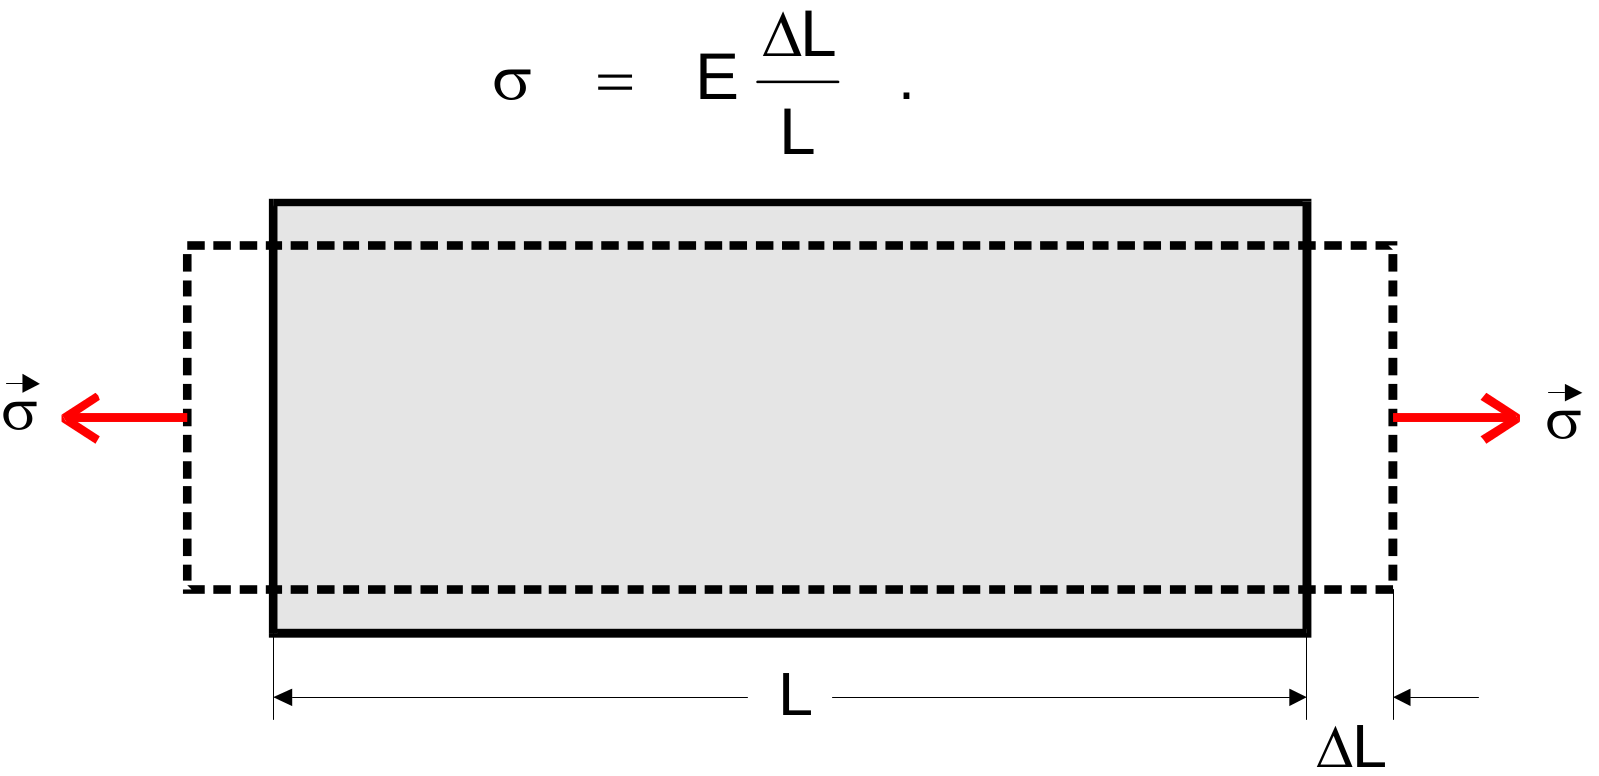
\includegraphics[width=0.9\textwidth]{spannung.png}
  \caption{Auswirkung einer Normalspannung auf eine stabförmige Probe \cite{sample} .}
  \label{fig:Spannung}
\end{figure}
Hierbei ist E der Elastizitätsmodul der eine Materialkonstante ist.
\subsection{Biegung bei einseitiger Einspannung}
In der Abbildung \ref{fig:Einseitige_Einspannung} ist, die schematische Darstellung einer Biegung bei einseitiger
Einspannung zu sehen.
\begin{figure}
  \centering
  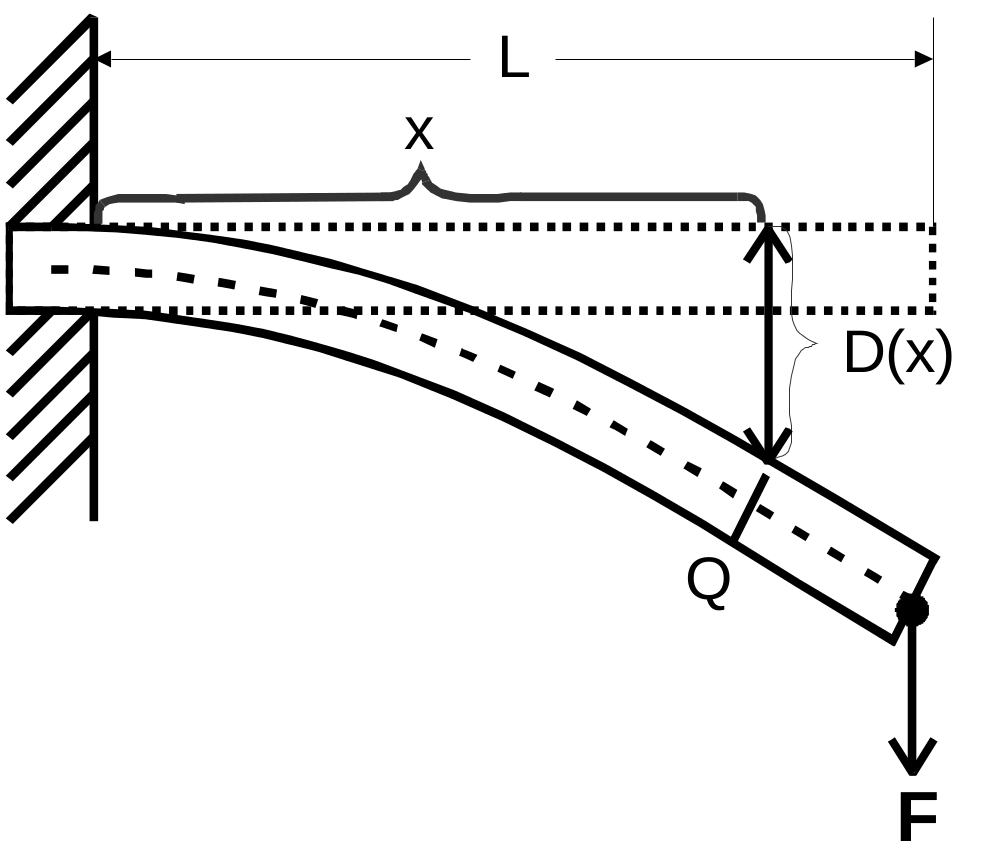
\includegraphics[width=0.5\textwidth]{einseitige.png}
  \caption{Schematische Darstellung der Biegung bei einseitiger Einspannung \cite{sample} .}
  \label{fig:Einseitige_Einspannung}
\end{figure}
Die Durchbiegung $D(x)$ lässt sich ermitteln indem man die Drehmomente aufstellt.
Bei der Biegung wird der eine Teil des Stabs gestaucht und der andere Teil gestreckt.
Der Teil der Spannungsfrei ist, wird neutrale Faser genannt und ist in Abbildung \ref{fig:Einseitige_Einspannung}
durch eine gestrichelte Linie angedeutet. Die wirkenden Kräfte an der stelle
$Q$ sind in Abbildung \ref{fig:Drehmomente} dargestellt.
\begin{figure}
  \centering
  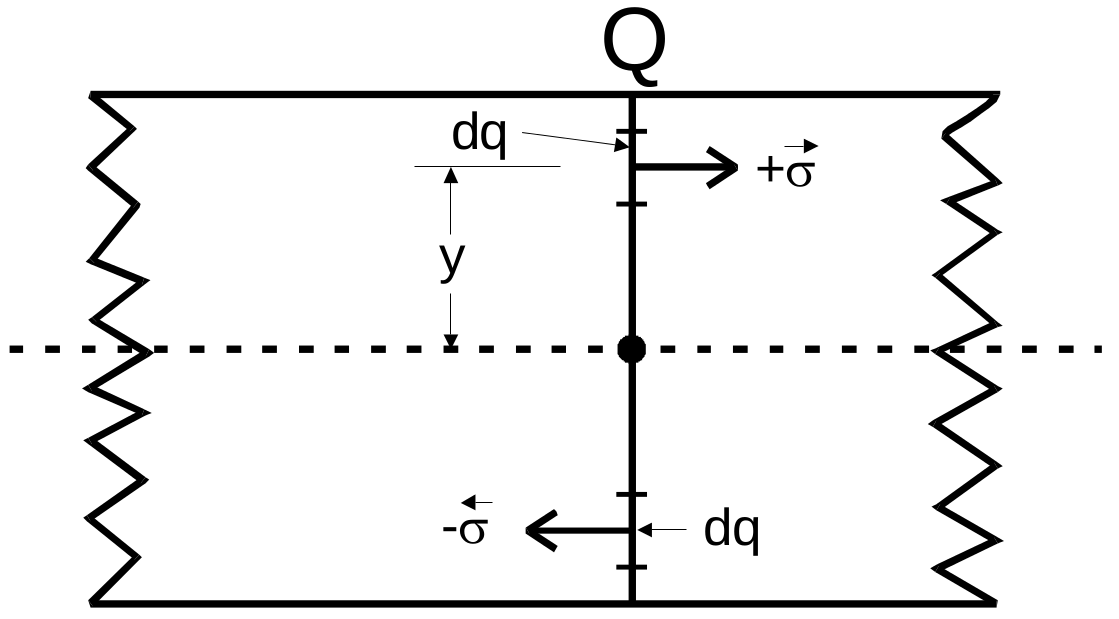
\includegraphics[width=0.5\textwidth]{Drehmomente.png}
  \caption{darstellung der Drehmomente bei Q \cite{sample} .}
  \label{fig:Drehmomente}
\end{figure}
 Die entgegengesetzten Druck- und
Zugspannungen sind vom betrag gleich. Mit \eqref{eqn:moment} lässt sich das Drehmoment $M_\sigma$
berechnen.
\begin{equation}
  M_\sigma=\int_Q y\sigma(y)\text{d}q
  \label{eqn:moment}
\end{equation}
Es stellt sich das Gleichgewicht
\begin{equation}
  M_F=M_\sigma
\end{equation}
ein. $M_F$ ist hierbei das durch die Gewichtskraft $F$, des angehängte Gewichts,
entstehende Drehmoment
und ist gegeben durch
\begin{equation}
  M_F=F(L-x)
\end{equation}
Das Gleichtgewicht ist also
\begin{equation}
  \int_Q y\sigma(y)\text{d}q=F(L-x)
\end{equation}
Die Normalspannung ist dur das Hookesche-Gesetz gegeben und ist mit einer Näherung
für geringe Kruvenkrümmungen
\begin{equation}
  \sigma(y)=E\frac{y}{R}=Ey\frac{\text{d}^2D}{\text{d}x^2}\;.
\end{equation}
so dass sich das Gleichgewicht als
\begin{equation}
  E\frac{\text{d}^2D}{\text{d}x^2}\int_Q y^2\text{d}q=F(L_x)
\end{equation}
schreiben lässt. Das Flächenträgheitsmoment $I$ ist gegeben durch
\begin{equation}
  I=\int_Q y^2 \text{d}q(y)\;.
  \label{eqn:Flaechentaegheitsmoment}
\end{equation}
Wird Gleichung \eqref{eqn:Flaechentaegheitsmoment} integriert, erhält man die Gleichung für die Durchbiegung
in abhängigkeit zu Abstand
\begin{equation}
  D(x)=\frac{F}{2EI}\left(Lx^2-\frac{x^3}{3}\right)\;\;\;\;(0\le x \le L)\,.
\end{equation}
\subsection{Biegung bei beidseitiger Auflage}
Da beide Enden des stabes aufliegen, greift nun die Kraft $\frac{F}{2}$ an.
Zu sehen ist eine schematische Darstellung in Abbildung \ref{fig:Beidseitige_Einspannung}
\begin{figure}
  \centering
  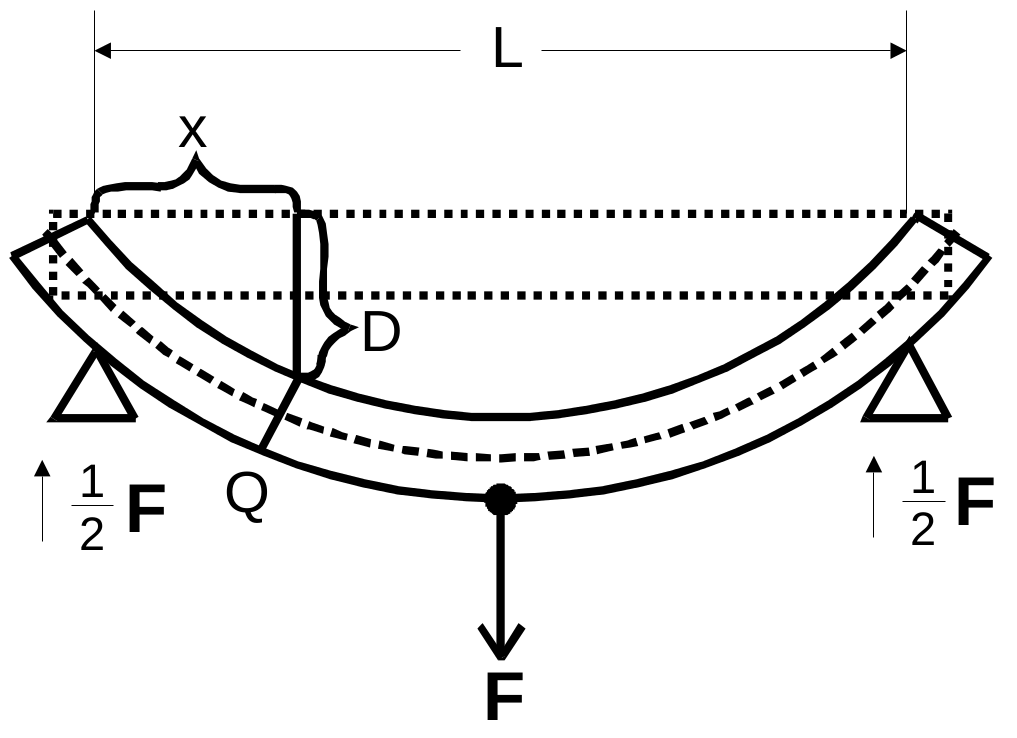
\includegraphics[width=0.5\textwidth]{Beidseitige_Einspannung.png}
  \caption{darstellung der Drehmomente bei Q \cite{sample} .}
  \label{fig:Beidseitige_Einspannung}
\end{figure}
Für die Drehmomente gelten nun
\begin{align}
  \frac{\text{d}^2D}{\text{d}x^2}=&-\frac{F}{EI}\frac{x}{2}\;\;(\text{für}\;0\le x \le \frac{L}{2}\\
  \frac{\text{d}^2D}{\text{d}x^2}=&-\frac{1}{2}\frac{F}{EI}(L-x)\;\; (\text{für}\; \frac{L}{2} \le x \le L)
\end{align}
und damit für die Durchbiegung
\begin{align}
  D(x)=&\frac{F}{48EI}\left(3L^2x-4x^3\right)\;\;(\text{für}\;0\le x \le \frac{L}{2})\\
  D(x)=&\frac{F}{48EI}\left(4x^3-12Lx^2+9L^2x-L^3\right)\;\; (\text{für}\; \frac{L}{2} \le x \le L).
\end{align}
\cite{sample}

\newpage
\section{Durchführung}
\label{sec:Durchführung}
\begin{figure}
  \centering
  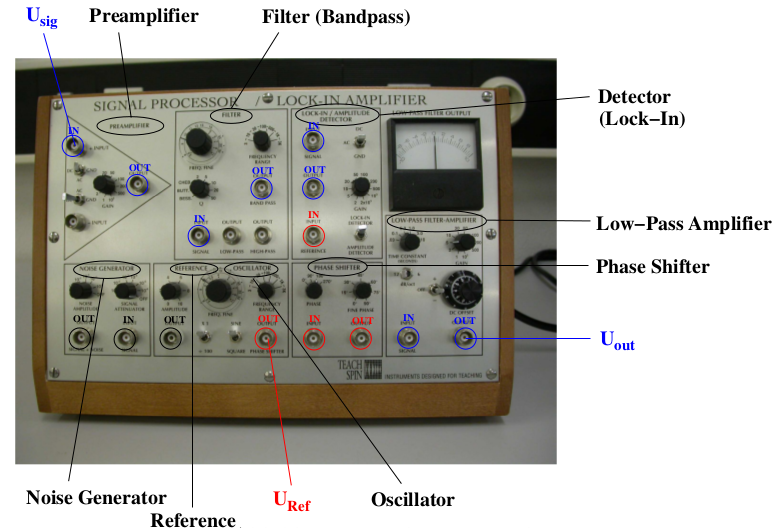
\includegraphics[width=0.8\textwidth]{verstaerker.png}
  \caption{Modularer Lock-In-Verstärker\cite{sample}.}
  \label{fig:verstaerker}
\end{figure}

{Es wird ein modularer Lock-In-Verstärker verwendet, welcher sich aus} folgenden
Elementen (auch in Abbildung \ref{fig:verstaerker} zu sehen) zusammensetzt:
Vorverstärker, Bandpassfilter, Phasenschieber, Funktionsgenerator, Rausch-Generator,
Tiefpass-Verstärker und Amplituden-/Lock-In-Detektor.

Zunächst werden die Signale des Funktionsgenerators mit Hilfe eines Speicheroszilloskops
überprüft. Dann wird nachfolgende Schaltung aufgebaut und der Rausch-Generator auf
OFF geschaltet.
\begin{figure}
  \centering
  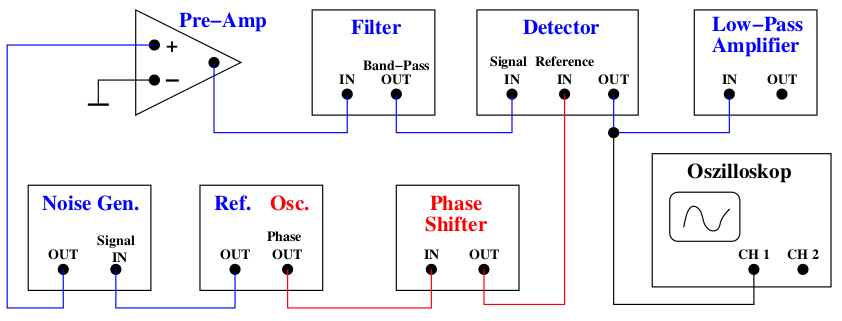
\includegraphics[width=0.8\textwidth]{schaltung.png}
  \caption{Schematischer Aufbau des Lock-In-Verstärkers\cite{sample}.}
  \label{fig:schaltung}
\end{figure}

Ein sinusförmiges Signal $U_\symup{sig}$ wird mit einem Referenzsignal
$U_\symup{ref}$ gleicher Frequenz gemischt und das Ausgangssignal für verschiedene
Phasen (je mit und ohne Integration durch den Tiefpass) graphisch dargestellt.
Desweiteren wird die Ausgangsspannung in Abhänigkeit der Phasenverschiebung
$\Delta\Phi$ gemessen.
Im nächsten Schritt werden diese Messungen wiederholt, jedoch mit eingeschaltetem
Rausch-Generator, sodass das Eingangssignal verrauscht ist.
\begin{figure}
  \centering
  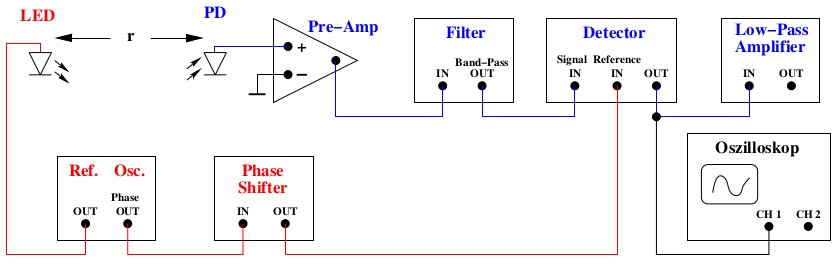
\includegraphics[width=0.8\textwidth]{photodetektor.png}
  \caption{Schematischer Aufbau der Photodetektorschaltung\cite{sample}.}
  \label{fig:photodetektor}
\end{figure}
Zuletzt wird eine Photodetektorschaltung nach Abbildung \ref{fig:photodetektor}
aufgebaut und die Lichtintensität der Leuchtdiode (LED) in Abhänigkeit des Abstandes
r zwischen der LED und der Photodiode gemessen, sowie der maximale Abstand bestimmt,
bei dem das Licht noch nachgewiesen werden kann.

\section{Auswertung}
\label{sec:Auswertung}
Der rechte Ausgang des Referenc/Oscillator gibt es eine konstante Spannung
von $2.4\si{\volt}$ der linke Ausgang liefert eine variable Spannung die
als Rechteck oder sinusförmige Spannung abgegeben werden kann. Für die
Phasenverschiebung $\Phi=0,0,0,0,0$ sehen die Signale wie in den folgenden
Bildern aus.
\begin{figure}
  \centering
  \begin{subfigure}{0.48\textwidth}
    \centering
    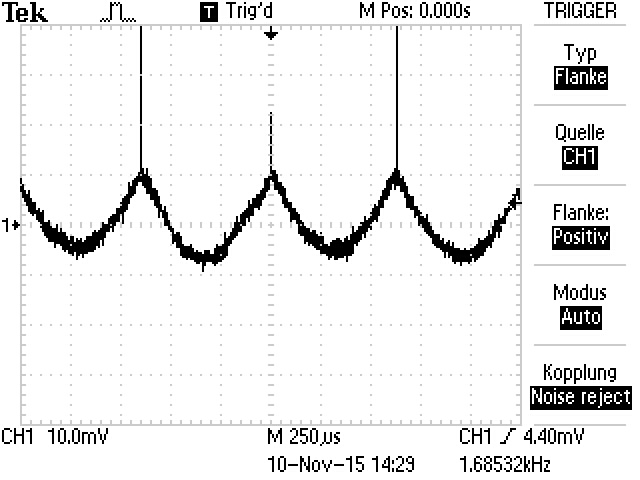
\includegraphics[height=0.75cm]{Bilder/or/or10.JPG}
    \caption{Phasenwinkel 10.}
    \label{fig:or10}
  \end{subfigure}
  \begin{subfigure}{0.48\textwidth}
    \centering
    %\includegraphics[height=0.75cm]{/pep.pdf}
    \caption{phasenwinkel 100.}
    \label{fig:pep2}
  \end{subfigure}  \centering
    \begin{subfigure}{0.48\textwidth}
      \centering
      %\includegraphics[height=0.75cm]{/pep.pdf}
      \caption{phasenwinkel 150.}
      \label{fig:pep2}
    \end{subfigure}
  \centering
  \begin{subfigure}{0.48\textwidth}
    \centering
    %\includegraphics[height=0.75cm]{/pep.pdf}
    \caption{phasenwinkel 190.}
    \label{fig:pep2}
  \end{subfigure}
  \begin{subfigure}{0.48\textwidth}
    \centering
    %\includegraphics[height=0.75cm]{/pep.pdf}
    \caption{phasenwinkel 280.}
    \label{fig:pep2}
  \end{subfigure}
\end{figure}
Wenn das Ausgangssignal über den Tiefpass für $\Phi=$ integriert wird sieht das
Signal aus wie in dem folgenden Bild.
\begin{figure}

\end{figure}
Die Messwerte Aus der Messung ohne Rauschen sind in folgender Tabelle aufgelistet
\begin{table}
  \centering
  \begin{tabular}{c c}
    \toprule
    $Spannung/V$  &  Phasenwinkel $\phi$\\
    \midrule
    24.8  &    0  \\
    22.8  &   30  \\
    15.7  &   60  \\
    12.0  &   90  \\
     5.7  &  120  \\
     1.3  &  150  \\
     0.8  &  180  \\
     3.2  &  210  \\
    10.4  &  240  \\
    14.2  &  270  \\
    20.6  &  300  \\
    24.8  &  330  \\
    25.0  &  360  \\
   \bottomrule
 \end{tabular}
 \caption{Differentialquotienten.}
 \label{tab:Diffquo}
\end{table}

\section{Diskussion}
\label{sec:Diskussion}
Die Fit Parameter der ersten Messung haben einen kleinen Fehler, der Weniger als
$5\%$ aus macht. Die Parameter zum Fit der zweiten Messung haben relativ
große Fehler von bis zu 50\%. Wie erwartet steigt der Dampfdruck mit
höheren Temperaturen, da die einzelnen Moleküle im Durchschnitt mehr
Energie haben. Abweichungen in den beiden Messreihen lassen sich dadurch erklären,
dass sich nicht immer ein Gleichgewicht eingestellt hat, wenn die Messwerte
abgelesen werden. Ein Anstieg desInnendrucks der Apparatur nach dem Schließen des
Absperrhahns zeigt, dass diese nicht ganz dicht war, was auch zu Messungenauigkeiten
geführt haben kann. Da die innere Verdampfungswärme viel größer als die äußere
Verdampfungswärme ist, lässt sich daraus schließen, dass die Überwindung der molekularen
Bindungen den Großteil der Verdampfungswärme aus macht. Wenn man die
Temperaturabhägigkeit der Verdampfungswärme betrachtet wird klar, dass nur die
Variante mit der positiven Wurzel aus
Abbildung \ref{fig:fit3} Sinn ergibt, da die Verdampfungswärme beim kritischen
Punkt null sein muss.  Nur so ist es möglich, das Flüssigkeits- und Gasphase
gleichzeit koexistieren. Auch weicht der Wert für die Verdampfungwärme in
Abbildung \ref{fig:fit4} zu stark ab.


\printbibliography

\end{document}
